\documentclass[]{article}

\usepackage[utf8]{inputenc}
\usepackage{amsmath}
\usepackage{amssymb}
\usepackage{amsthm}
\usepackage{amsfonts}
\usepackage{mathtools}
\usepackage[margin=1.6cm]{geometry}
\usepackage[most]{tcolorbox}
\usepackage{graphicx}
\usepackage{capt-of}
\usepackage{adjustbox}
\usepackage{listings}
\usepackage[hidelinks]{hyperref}
\usepackage{cleveref}
\usepackage{siunitx}
\usepackage{subcaption}
\usepackage{siunitx}
\usepackage{biblatex}
\addbibresource{references.bib}
\usepackage[section]{placeins}
\usepackage{float}


\title{The suprising intutition of the Hopfield network}

\begin{document}
\maketitle

\section{Abstract}
The Hopfield network is an important model for understanding the mechanisms behind associative memory, and is an important basis for many state-of-the-art methods in artifical neural networks. In this paper we utilize numerical and analytical methods to show how the Hopfield network with a Hebbian learning rule always converges toward a local equilibrium. By borrowing the concept of energy from physics, we will build an intuitve understanding for how the Hopfield network may be used to model associative memory.  
\section{Introduction}
Sensor fusion is commonly used in robotics and autonomous systems to fuse multiple sources of information (sensors) to create better estimates of a systems state. Any single source may only contains partial information and may only perform well in a few scenarios. However, with enough sources we might still be able to create solid estimates by updating a common belief.  
By considering neurons in the brain as sources of information, the brain may be thought of as a large scale sensor fusion system.

The aim of this paper is to investigate whether it is possible to predict head direction of a mouse by considering the spike-train of different cells in the brain, and see how well a sensor fusion framework may explain how multiple cells can be combined to create one head direction estimate. 
\section{Method}

\subsection{The Hopfield Network}
The Hopfield Network is a simple fully-connected neural network, i.e. all neurons are connected to eachother. Each neuron is either on (firing) or off (not firing) encoded as positive and negative values
$$s_i \in \{1, -1\}$$ where $s_i$ is the state of neuron $i$.
The connection between two seperate neurons is weighted, and there are no self-connections. The weight matrix can be initialized to store different memories 
\begin{align}
    \mathbf{W} &= {\bar{\mathbf{W}}} - diag^{-1}(\bar{\mathbf{W}}) & \bar{\mathbf{W}} &= \sum_{m=1}^M \mathbf{V}^{(m)} (\mathbf{V}^{(m)})^T 
\end{align} where $\mathbf{V^{(m)}}$ is a column vector storing the pattern for memory $m$.
Each element in the weight matrix then corresponds to
\begin{equation}
    w_{ij} = \begin{cases}
        \sum_{m=1}^M v_{i}^{(m)} v_{j}^{(m)} & \forall i \neq j \\
        0 & \forall i = j
    \end{cases}
\end{equation}
The network states can then be updated by using the update rule
\begin{align}
    s_i &= sign(h_i) & h_i = \sum_{j} w_{ij} s_j \iff \mathbf{H} = \mathbf{W} \mathbf{S}
\end{align}
The neurons can either be updated using an asynchronous or synchronous approach. With asynchronous updating, the neurons are updated in random order at different times, while with syncrhonous updating they are updated all at once. To mimick biological systems, we use asynchronous updating.

\subsection{Simulating the Hopfield network}
The Hopfield network was implemented and simulated in MATLAB.

\subsection{Creating patterns from QR codes}




\section{Results}

\subsection{Stability of Hopfield Network}
\begin{figure}[H]
    \centering
    \begin{subfigure}{0.49\textwidth}
        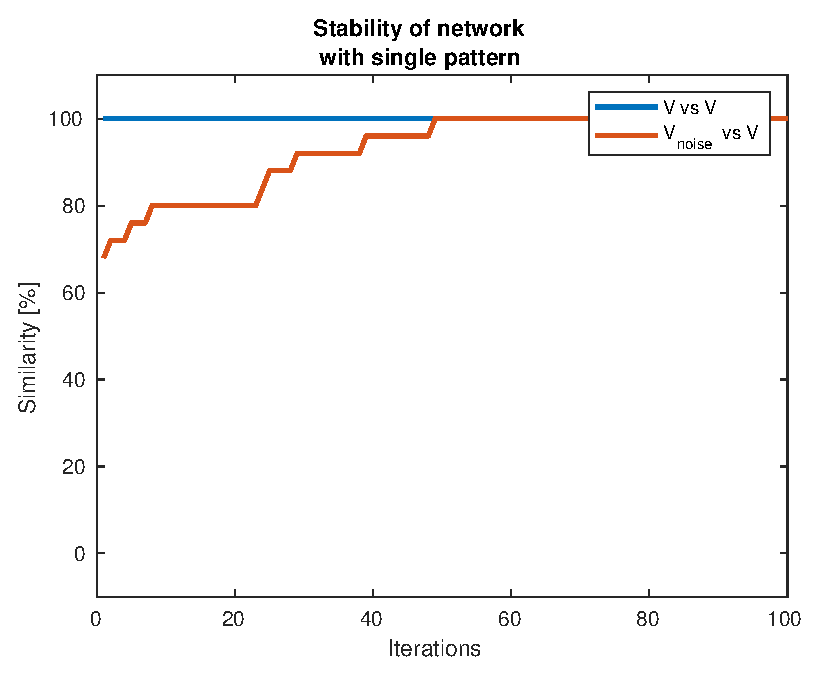
\includegraphics[width=\textwidth]{figs/stable}
        \caption{By initializing the network to the stored pattern, the network will remain in an equilibrium. The network will never deviate from this state without external interference.If the network is initialized to a noisy state, the network will converge towards the stored pattern.}
    \end{subfigure}
    \begin{subfigure}{0.49\textwidth}
        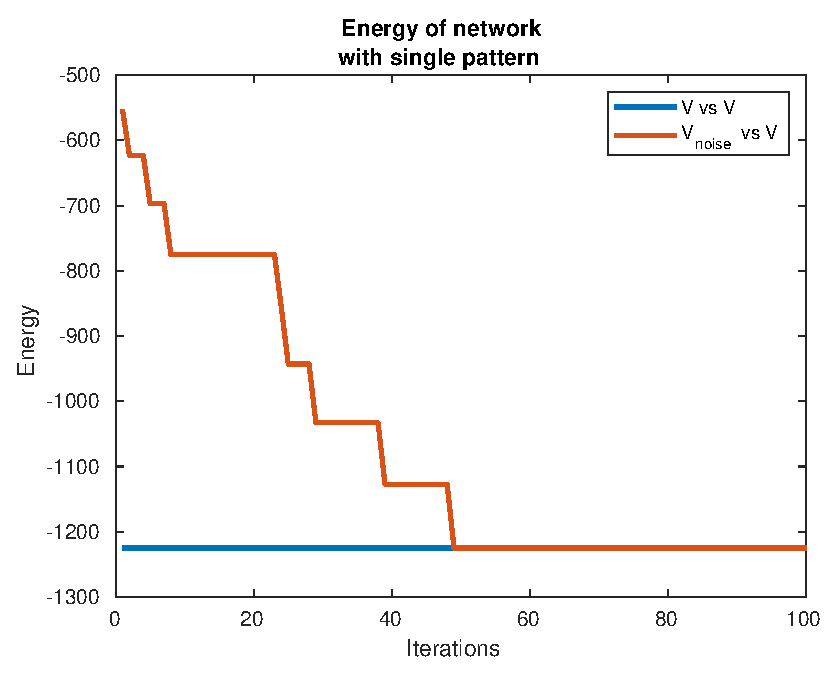
\includegraphics[width=\textwidth]{figs/stable-energy}
        \caption{With a single stored pattern, the energy will converge towards the lower limit according to \cref{eq:energy-limits}. In this case with 50 neurons, the lower limit os $-\frac{50*\times 49}{2} = -1225$}.
    \end{subfigure}
    \caption{Initializing a Hopfield network with a single stored pattern ($N = 50$) will cause the network to converge towards the stored pattern.}
    \label{fig:stable}
\end{figure}
To test whether the Hopfield network is stable after reaching an equilibrium we simulated the Hopfield network storing a random pattern using $N=50$ neurons. We initialized the network to the stored pattern, once with and once without noise added, as shown in \cref{fig:stable}. The network remains stable at the equilibrium point, and it will converge towards the equilibrium if not perfectly intialized. With a single pattern stored, the energy will converge toward the lower limit expressed in \cref{eq:energy-limits}.

\subsection{Storing multiple patterns}
\begin{figure}[H]
    \centering
    \begin{subfigure}{0.49\textwidth}
        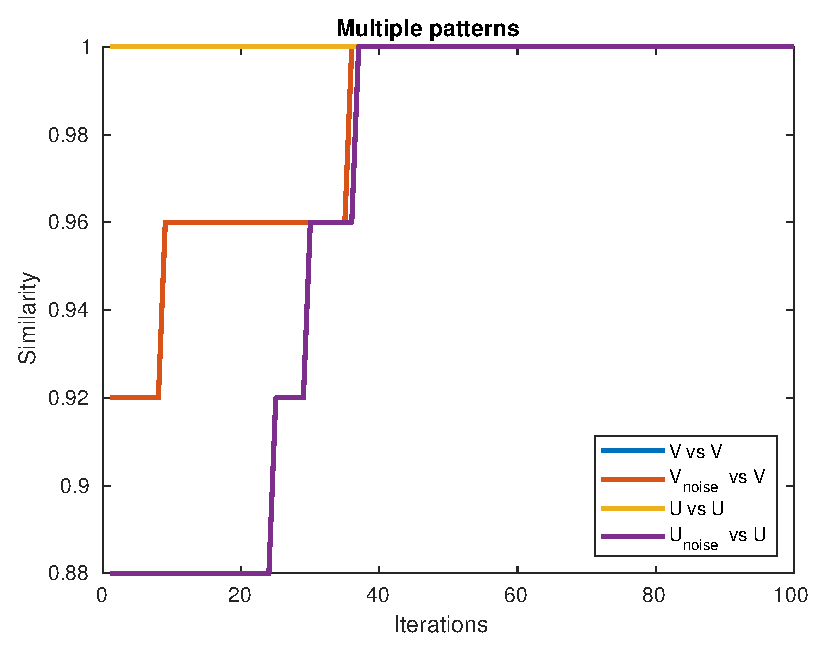
\includegraphics[width=\textwidth]{figs/multiple-patterns.eps}
        \caption{By initializing the weight matrix $\bf W$ with multiple patterns, the network is able to restore multiple different patterns. The amount of memories and noise the network is able to handle, depends on complex the pattern is (number of neurons) and how similar the patterns are. If two stored patterns only differ by one bit, the network may recall the wrong memory if noise is involved. }
        \label{fig:multiple-similarity}
    \end{subfigure}
    \begin{subfigure}{0.49\textwidth}
        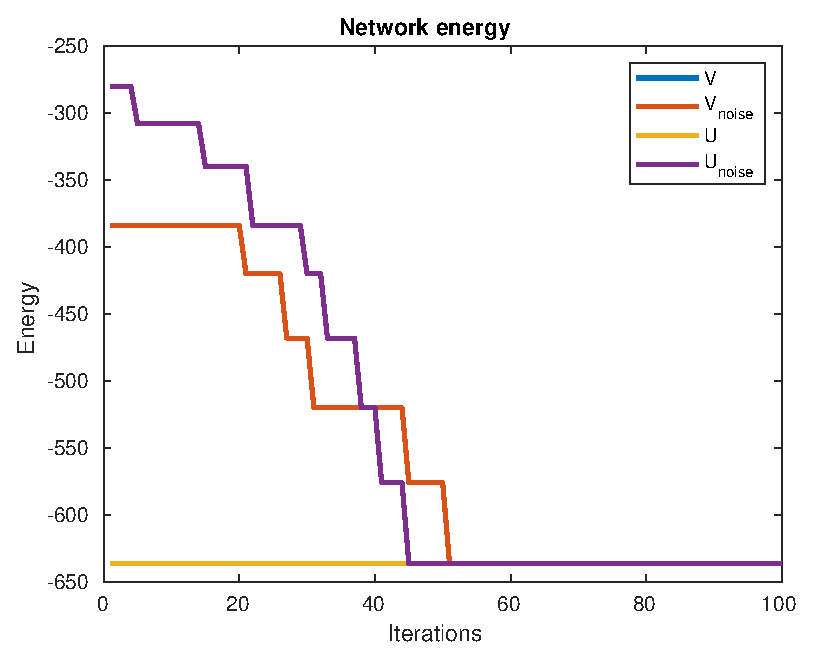
\includegraphics[width=\textwidth]{figs/multiple-patterns-energy.eps}
        \caption{The network will always move in the direction of least resistance such that the overall energy decrease, similar to how a ball always will roll downwards into a valley unless there are external forces interfering. Each stored memory corresponds to a local minimum which can be thought of as valleys, and as long as the network is initialized in the correct valley, it is able to reconstruct the state from memory.}
        \label{fig:multiple-energy}
    \end{subfigure}
    \caption{Simulating the Hopfield network with multiple stored patterns.}
    \label{fig:multiple}
\end{figure}
To test whether the network remains stable even with multiple patterns stored, we simulated a new network storing two uncorrelated random patterns ($N=50$). We simulated using both patterns as initial conditions as well as simulating with and without noise. In total we ran 4 simulations and the results are shown in \cref{fig:multiple}. The states converged towards the correct pattern in all cases, and remains stable at the equilibrium. The energy in the equilibrium, as shown in \cref{fig:multiple-energy}, was half the networks lower limit in \cref{eq:energy}.
 

\subsection{Reconstructing partially lost QR codes from memory} \label{sec:qr-codes}
To better visualize the Hopfield networks ability to store and restore patterns, we constructed a Hopfield network to store QR-codes. We stored two QR-codes in the network and initialized the network with only partial information. \cref{fig:qr-codes} shows how the network was able to restore the correct QR code from memory, while \cref{fig:qr-codes-stability} shows how the network remains stable after reaching the equilibrium.
\begin{figure}[H]
    \centering
    \begin{subfigure}{0.49\textwidth}
        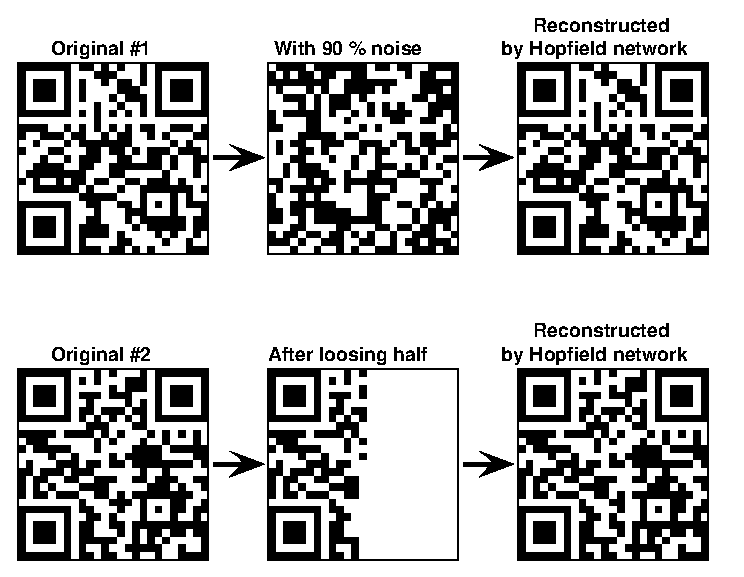
\includegraphics[width=\textwidth]{figs/qr-code}
        \caption{The QR-code contains information encoded within the patterns. A QR decoding app, either online or on a smartphone, can be used to decode the "hidden" message. Using the hopfield network we are able to reconstruct a destroyed QR-code from memory.}
        \label{fig:qr-codes}
    \end{subfigure}
    \begin{subfigure}{0.49\textwidth}
        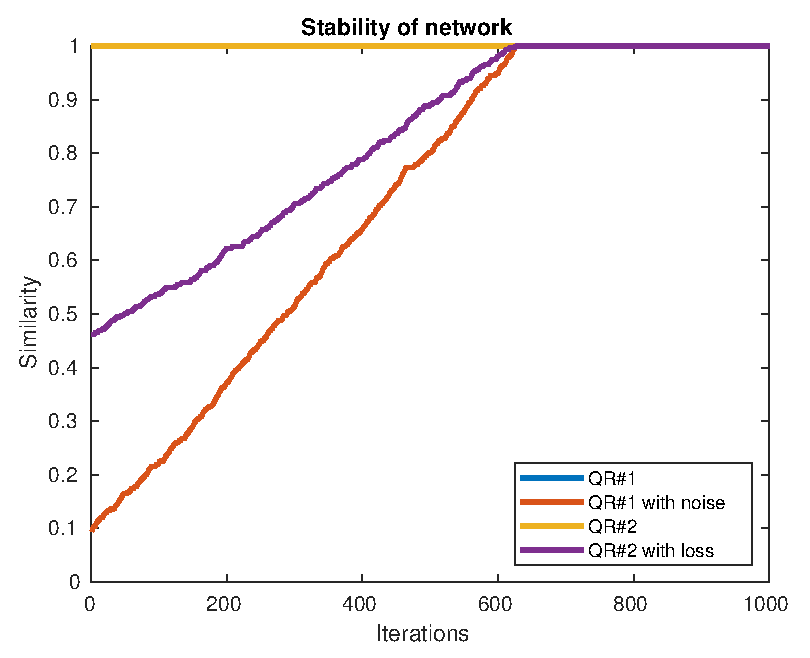
\includegraphics[width=\textwidth]{figs/qr-code-sim}
        \caption{The similarity between the current state of the network and the original QR-code we want it to reconstruct.}
        \label{fig:qr-codes-stability}
    \end{subfigure}
    \caption{By applying the Hopfield network to a very noisy QR-code we are able to reconstruct the original. By using any QR-code reader we are able to decode the left and right QR-codes, while the middle ones contains too much noise. The same hopfield network was used.}
\end{figure}

\subsection{Inverting patterns}
According to the weights, \cref{eq:weights}, the Hopfield network only stores patterns and not the actual values in the memories. A pattern $\bf V$ and its inverse $\bf \bar{V} = -1 \times \bf V$ would yield the exact same weight matrix. For each stored memory there should be two equilibrium states, one for $\bf V$ and one for $\bf \bar{V}$. To test wheter this truly was the case, we used the same Hopfield network as in \cref{sec:qr-codes} and initialized the states to the second QR code, but inverted. We ran another simulation using the QR-code with two-thirds of its bits inverted. As can be seen from the results in \cref{fig:inverted-qr} both cases caused the Hopfield network to reconstruct the inverted pattern, and not the one we originally created.
\begin{figure}[H]
    \centering
        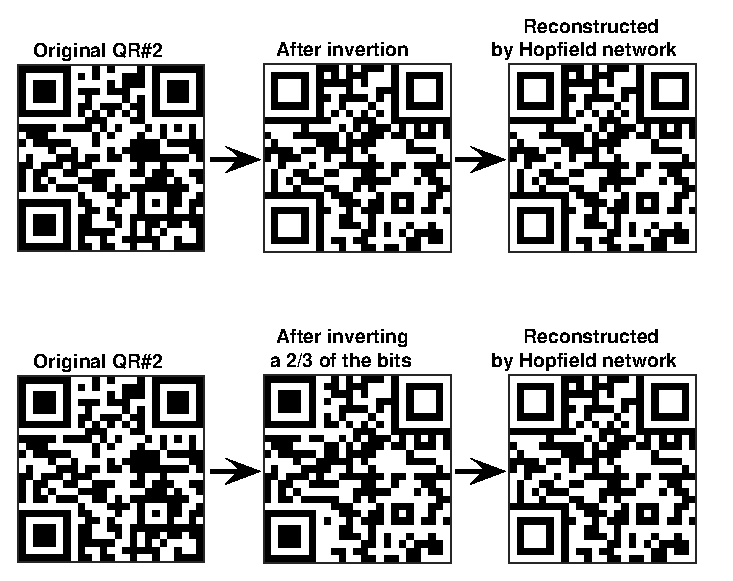
\includegraphics[width=0.4\textwidth]{figs/qr-inverted}
        \caption{The Hopfield network learns the patterns and the network is not able to distinguish between positive and negative values. The network is not only stable at the initial memories, but also when using the inverted patterns. This makes sense from a memory point of view, as we are able to distinguish objects purely based on patterns and shapes. An apple is an apple regardless of its color.}
        \label{fig:inverted-qr}
\end{figure}
\section{Discussion and conclusion}

From our empirical results we are able to verify the stability properties of the Hopfield network. The network is able to restore multiple different patterns from partial inputs, and is stable in the equlibrium points. Our empirical results cannot guarantee global stability, and it is difficult to draw good conclusions purely from a few simulated results. There are however a great deal of research on the stability of the Hopfield network, and the stability of the network have been mathematically proved using Lyapunov analysis. By considering the energy in \cref{eq:energy} as a Lyapunov candidate, it can be show that the energy is (nonstrictly) decreasing when using the update rule in \cref{eq:update} \cite{lyapnuv-stability}.

When simulating with multiple uncorrelated patterns the network energy lower limit from \cref{eq:energy-limits} appears to be roughly divided equally between the two patterns. The energy limits may therefore not only be used understand how the network is stable, but can also be used to quantify the capacity (i.e. the number of memories the network can store). How the energy is distributed does however depend on how similar the memories are. We can think of memories with a lot in common as creating smaller valleys within a larger valley, and thereby sharing some potential energy. Intuitively we should therefore be able to store as many memories as we can create valleys using the finite amount of discrete energy in the network.

The energy may also be used to quantify the robustness of the network. By considering the amount of work needed (in a physical sense) to move the state of the network from one memory to another, we can create a quantitative measure for how robust the network is to random perturbations. If the amount of energy required to move the state between two memories (i.e. the amount of work required to move the state out of one valley) is small, then noise in only a few bits may be enough to recall the wrong memory. Storing too many memories (i.e. having too many small valleys), or storing very similar patterns will therefore decrease the robustness.

Our results also showed that for each stored pattern, there are two equlibrium points - an original and an inverted pattern. In other words, the Hopfield network does not store the actual values of the stored patterns, but only whether any pair of neurons should be equal or not. This appears to be consistent with how we as humans are able to associate memories with objects regardless of specific details - an apple is an apple regardless of whether it is real or painted. 

There are however many limitations to the Hopfield network, and it is in no way a perfect model of the mechanisms behind memory in humans or animals. Nevertheless it helps us understand how a complex network of simple units (neurons) are able to recall memories, and many of its limitations have been solved in more modern approaches to ANNs.









\printbibliography
\appendix
\section{Proof of equation \ref{eq:energy}}\label{sec:proofenergy}
The third equality \cref{eq:energy-compact} is valid since 
\begin{equation*}
    trace(\bar{\mathbf{W}}) = \mathbf{S}^T diag^{-1}(\bar{\mathbf{W}})\mathbf{S}
\end{equation*}
The last equality, \cref{eq:energy}, comes from the fact that the trace of $\bar{\mathbf{W}}$ (\cref{eq:weights}) is the sum of the diagonal elements, and the diagonal elements of $\bar{\mathbf{W}}$ are given by
\begin{equation}
    \bar{w}_{ii} = \frac{1}{M} \sum_{m=1}^M (v_i^{(m)})^2 \equiv 1
\end{equation}
The trace of $\bar{\mathbf{W}}$ is therefore given by 
\begin{equation}
    trace(\bar{\mathbf{W}}) = \sum_{n=1}^N 1 = N
\end{equation}

\section{Matlab Code} \label{sec:matlab_code}
\lstinputlisting[breaklines=true,language=MATLAB]{../../project2.m}
\lstinputlisting[breaklines=true,language=MATLAB]{../../runSim.m}

\end{document}

